\documentclass[12pt,a4paper,openright]{article}
\usepackage[utf8]{inputenc}
\usepackage[spanish]{babel}
\usepackage{amsmath}
\usepackage{amsfonts}
\usepackage{amssymb}
\usepackage{subfigure}
\usepackage{enumerate}
\usepackage{graphicx}
\usepackage[left=2cm,right=2cm,top=2cm,bottom=2cm]{geometry}
\author{Jorge Benz Olguín Aguilar}
\title{Actividad 3}
\begin{document}
\maketitle
\section*{Introducción}

En esta actividad de elaboramos nuestro primer programa en Fortran para estudiar una función, que posee todas sus derivadas de orden superior. \\


En matemáticas, una serie de Taylor es una aproximación de funciones mediante una serie de potencias o suma de potencias enteras de polinomios como $( x-a )^n$ llamados términos de la serie, dicha suma se calcula a partir de las derivadas de la función para un determinado valor o punto a suficientemente derivable sobre la función y un entorno sobre el cual converja la serie. Si esta serie está centrada sobre el punto cero, $a=0$, se le denomina serie de McLaurin \\


$$
f(a)+\frac{f^1(a)}{1!}(x-a)+\frac{f^2(a)}{2!}(x-a)^2+\frac{f^3(a)}{3!}(x-3)^3 
$$



\section*{Actividades a realizar}


Iniciando con ese programa, modifícalo para:
encontrar los ceros de la función sin(x), i.e., el conjunto de x, para los cuales f(x)=0. Llama a estos puntos x0, x1, x2.
Si, utilizamos la aproximación de primer orden (la secante), de la derivada f'(x(i)) = (f(x(i+1) - f(x(i)))/dx. Por favor ubica los valores extremos de sin(x), los puntos xm0, xm1,  donde f'(x)=0.
Ya vimos que la Serie de Taylor para f(x) = sin(x) alrededor de x=0, esta dada por la expresión 

$$\sin(x)\approx x-\frac{x^3}{3!}+\frac{x^5}{5!}-\frac{x^7}{7!}
$$




\begin{verbatim}

! Este programa calcula la función Sin(x) en el intervalo [0, 2 pi]
! Definimos el nombre del programa Fortran. Le damos el mismo nombre que el 
! programa fuente sinfunct.f90
 
program sinfunct
! Tres espacios de sangría
! No suponemos nada
  implicit none
 
! Definimos todas la variables que vamos a utilizar y su tipo
  integer :: i, npts ! npts es el número de puntos en el intervalo [0,2pi]
  real :: x, f_x,dx  ! La variable, una función f(x) y el incremento dx
  real, parameter :: pi = 4.0 * atan (1.0) ! Dejamos que la máquina calcule pi
 
  print *,  'Dame el número de puntos en el intervalo npts= '
  read(*,*) npts
 
  dx = (2.0 * pi) /float(npts) ! dx es el incremento en el eje x
  write(*,*) 'dx= ', dx
 
  x = 0.0 ! Es el límite inferior del intervalo de interés
  ! Comenzaremos evaluando f(x) desde x=0, y debemos incluir también x=2*pi
 
! Inciamos un "loop", notemos la sangría dentro del loop. !
  do i = 1, npts+1, 1 
     x = dx * float(i-1)
     f_x = sin(x)
     write(*,*) i, x , f_x
enddo
! termina el loop
end program sinfunct 
! termina el programa

\end{verbatim}

\begin{large}
A partir del codigo anterior realizamos lo siguiente 
\end{large}

\begin{verbatim}

!programa fuente sinfunct

program sinfunct
  implicit none

  !definimos todas las variables
  
  integer :: i,npts ! npts es el numero de puntos en el intervalo
  ! [0,2pi]
  real :: x, f_x,f__x, dx, sintaylor !la variable, una funcióm F(x) y el incremento dx
  real, parameter :: pi = 4.0*atan(1.0) !dejamos que la maquina calcule
  !pi
  real, parameter :: epsilon = 1.0E-6
  
  print *, 'dame el número de puntos en el intervalo npts='
  read(*,*) npts
  dx=(2.0 * pi)/float(npts) !dx es el incremento en el eje x
  write(*,*) 'dx=',dx
  
  x=0.0
  
  open(unit=11, file='seno.dat')
  
  !iniciamos un loop, notemos la sangria dentro del loop
  
  do i=1, npts+1,1
     x=dx*float(i-1)
     f_x=sin(x)
     write(11,*) x,f_x
     if (abs(f_x).le. epsilon) write(*,*)'x=',x,'Cero de la función'
  enddo

  close(11)

  open(unit=11, file='coseno.dat')

  do i=1, npts+1,1
     x=dx*float(i-1)
     f__x=cos(x)
     write(11,*) x, f__x
     if(abs(f__x).le.epsilon)write(*,*)'x=',x,'Es un cero de la deriva&
          &da'
  enddo
  close(11)

  do i=1,1,1
     x=pi/8.0
     sintaylor=x-(x**3.0)/(3.0*2.0)
     write(*,*)'porcentaje de error con respecto a taylor',(1&
          &-(sintaylor/sin(x)))*100, '%'
  enddo
  
     !termina el loop

end program sinfunct
!termina programa

\end{verbatim}

A partir de lo cual se calculo el seno y coseno para diferentes puntos, así como una aproximación por medio de la serie de Taylor.  \\
Las siguientes gráficas son una muestran de lo que el codigo calcula para una cantidad de puntos determinada.   \\ \\ 

\begin{figure}[htb]
\centering
\subfigure[Gráfica Seno]{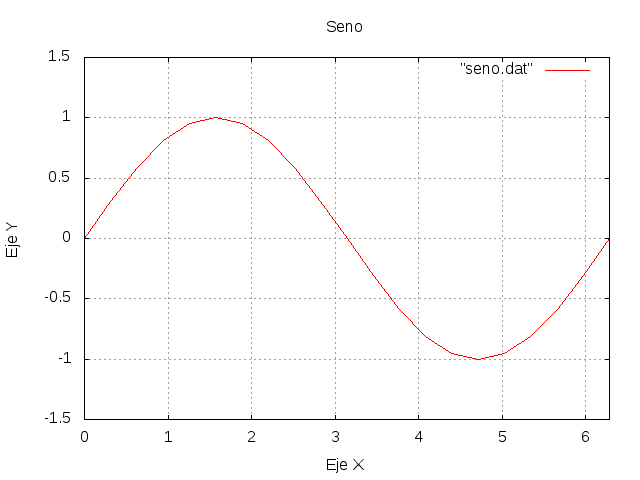
\includegraphics[scale=0.45]{seno.png} } \hspace{10mm}
\subfigure[Gráfica Coseno]{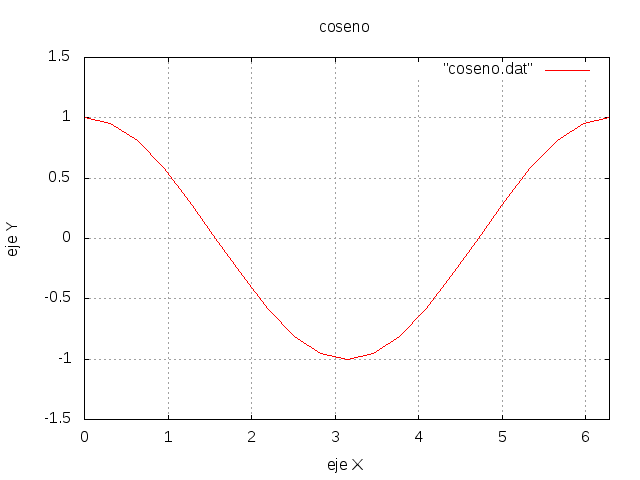
\includegraphics[scale=0.45]{Coseno.png} } 
\caption{Comparación en Gráficas diferentes} 
\end{figure} 


Para la realización de las gráficas utilizamos el programa Gnuplot, el cual es un graficador en base a comandos, la gráfica de comparación es sencilla y las instrucciones basicas, pero muestran el objetivo final de la practica.

\begin{figure}[htb]

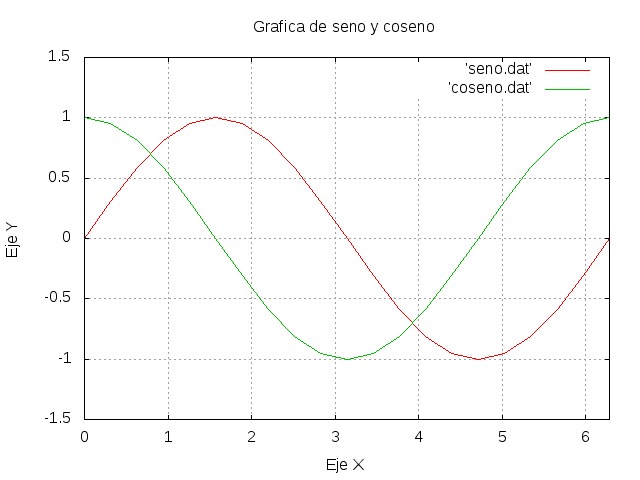
\includegraphics[scale=1]{senoycoseno.png} 
\caption{Comparación de seno y coseno en la misma gráfica}
\end{figure}



\end{document}